En esta práctica se aborda el problema de localización de un robot móvil. Se considera un robot con un sistema sensor, que tiene un cierto error de medición, y unas balizas, que son los puntos respecto a los que se toman las mediciones. 
En este caso, las balizas son a la vez los objetivos, es decir, describen la ruta que debe seguir el robot. Para esta simulación se calcula la predicción o modelo de la posición del robot, en base al movimiento que se realiza en los actuadores. 
No obstante, este movimiento tiene un cierto ruido, por lo que la posición real del robot dista de la posición ideal o estimada. Por tanto, se deben emplear las mediciones para corregir el modelo y ajustarlo a la realidad.


\section{Código Implementado}
El script proporcionado contiene muchas de las funciones necesarias, sin embargo, se debe implementar código para poder calcular la localización.

\subsection{Análisis}
Se implementan las siguientes características:
\begin{itemize}
  \item \texttt{Función de localización}: Dadas las balizas, el robot ideal, el robot real y las mediciones, se toma un punto de búsqueda a partir del cual se explora un área cuadrada comprendida entre -radio y radio, 
  usando un incremento indicado como parámetro. Se comprueban todas las posiciones posibles dentro de ese área, y se calcula la probabilidad de cada una en función de las mediciones del sensor y las posiciones de las balizas.
  Por último, se devuelve la posición con mayor probabilidad. Esta función se puede observar en la figura \ref{fig:localizacion_fun1}.
  \item \texttt{Localización inicial}: Para comenzar la localización, se debe determinar la posición en la que comienza el robot. \ref{fig:localizacion_inicial}.
  \item \texttt{Ajuste de la posición}: Mientras el robot se mueve, se debe verificar si la posición predicha es correcta, para ello se comprueba la probabilidad de las mediciones de los sensores respecto a la posición predicha.
  Se establece un umbral de error, que al ser superado causa un ajuste de la posición del modelo. Para ello, se emplea la función de localización descrita, tomando un radio de $2*error\_mediciones$. \ref{fig:localizacion_correccion}.
\end{itemize}

En la figura \ref{fig:localizacion_param} se observan algunos de los parámetros que se han indicado del script, más adelante se experimentará con ellos. 

\begin{figure}[htb]
  \centering
  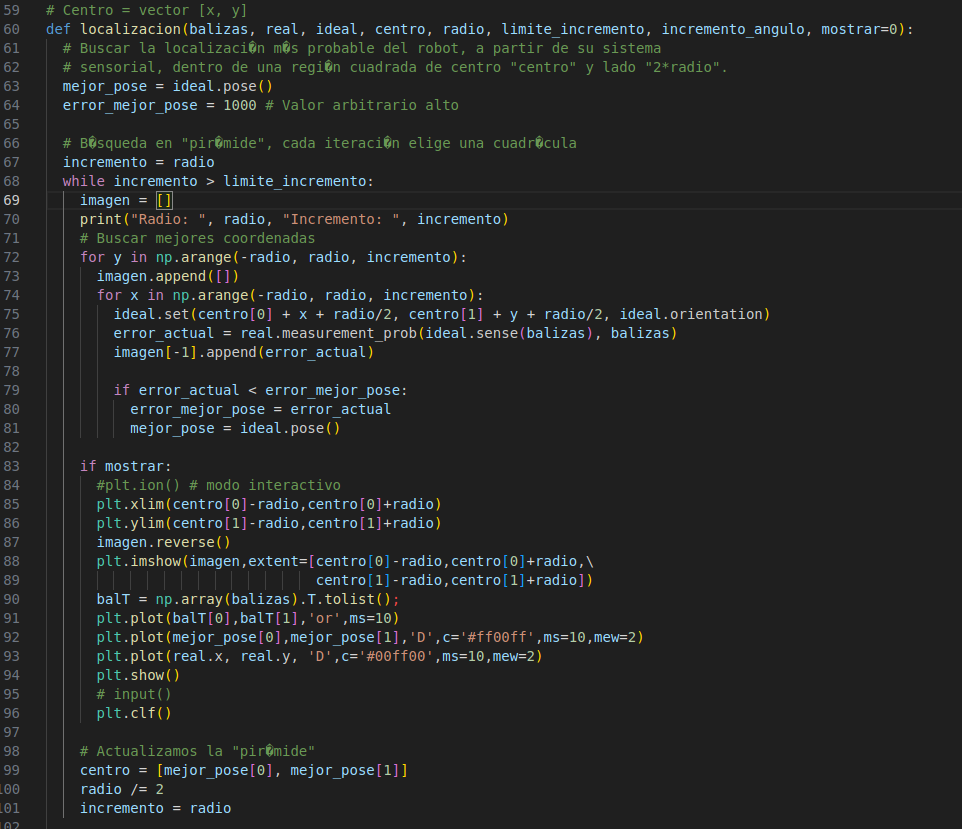
\includegraphics[width=1\linewidth]{images/localizacion1.png}
  \caption{Primera parte de la función de localización}
  \label{fig:localizacion_fun1}
\end{figure}
\begin{figure}[htb]
  \centering
  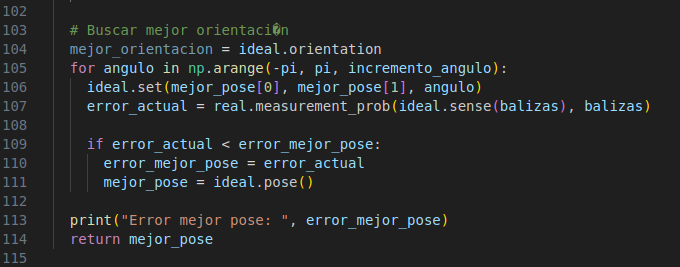
\includegraphics[width=.8\linewidth]{images/localizacion2.png}
  \caption{Fin de la función de localización}
  \label{fig:localizacion_fun2}
\end{figure}
\begin{figure}[htb]
  \centering
  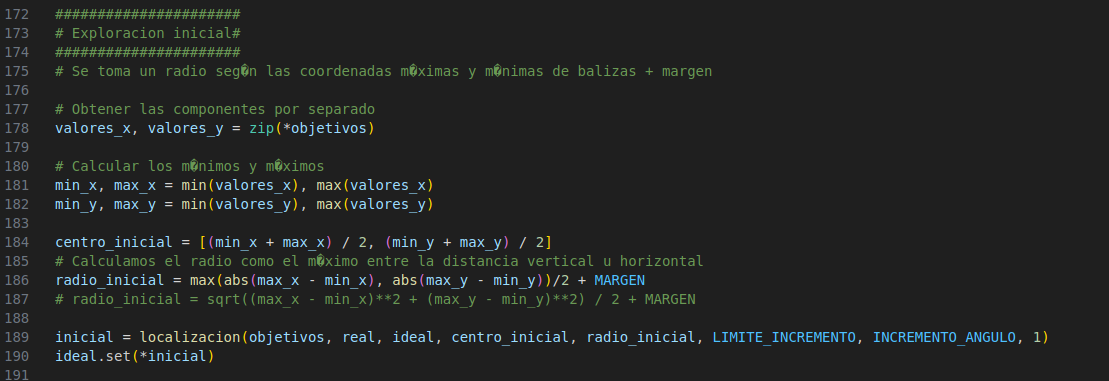
\includegraphics[width=1\linewidth]{images/localizacion5.png}
  \caption{Localización inical}
  \label{fig:localizacion_inicial}
\end{figure}
\begin{figure}[htb]
  \centering
  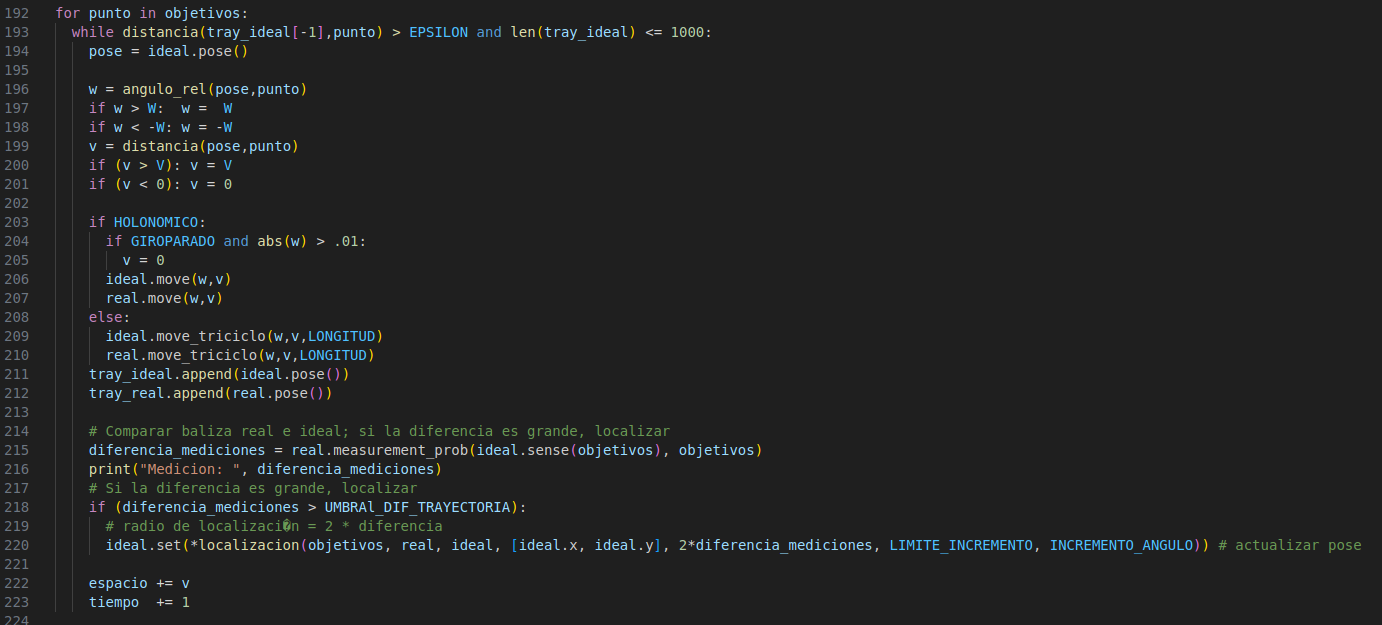
\includegraphics[width=1\linewidth]{images/localizacion6.png}
  \caption{Corrección de la posición}
  \label{fig:localizacion_correccion}
\end{figure}
\begin{figure}[htb]
  \centering
  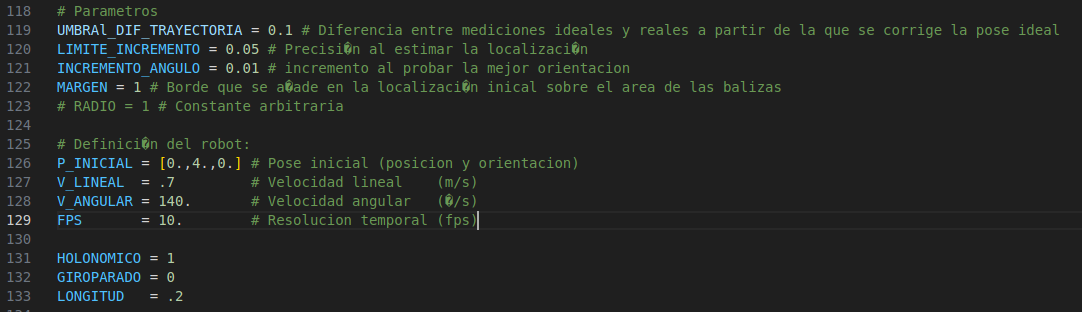
\includegraphics[width=1\linewidth]{images/localizacion3.png}
  \caption{Parámetros de la localización}
  \label{fig:localizacion_param}
\end{figure}

\subsection{Complejidad}
Los cálculos del algoritmo de localización se deben realizar al inicio, y luego cuando se supera el umbral de error. Por tanto, el rendimiento del programa dependerá del ruido en el movimiento, así como del ruido de los sensores, 
y principalmente, del umbral de error considerado. Un mayor umbral resulta en menos cálculos, mientras que un umbral menor requiere una mayor precisión, y por tanto, más cálculos. Se debe tener cuidado, puesto que un umbral demasiado bajo 
puede causar cálculos excesivos debido a los ruidos de sensores.

\bigskip Respecto a la función de localización, su complejidad depende del radio y el incremento considerado. Un menor incremento realiza un barrido más exhaustivo del área, pero requiere más cálculos. Por tanto, es importante elegir un valor que 
consiga un balance entre precisión y rendimiento.

%%%%%%%%%%%%%%%%%%%%%%%%%%%%%%%%%%%%%%%%%%%%%%%%%%%%%%%%%%%%%

\section{Mejoras}
En adición al comportamiento básico, se han implementado varias mejoras:
\subsection{Ajuste de la orientación} Además del ajuste de la posición, se implementa un cálculo similar para detectar la orientación (rotación) más probable. Se realiza un barrido entre $-\pi$ y $\pi$ con un incremento dependiente de un parámetro, y se calcula la probabilidad de cada orientación en función de las mediciones y la posición previamente predicha. El código correspondiente se aprecia en la figura \ref{fig:localizacion_fun2}.
\subsection{Uso de incremento piramidal} En lugar del comportamiento descrito previamente, en el que se emplea un incremento constante para el barrido del área a estudiar, se emplea un algoritmo de barrido piramidal, en el que en cada iteración se divide el área en 4 cuadrantes,
estudiándose el centro de cada uno, y seleccionando el cuadrante con mayor probabilidad. Este proceso se repite hasta que los cuadrantes tienen un tamaño inferior a un límite establecido. El código correspondiente se muestra en la figura \ref{fig:localizacion_fun1}. Cabe destacar
que esta forma es mucho más eficiente para estudiar el área, puesto que se evitan cálculos innecesarios. Sin embargo, se puede perder un poco de precisión ya que es posible que se seleccione un cuadrante erróneo si el punto se sitúa en el extremo entre dos, debido a los ruidos.
\subsection{Cálculo de un radio inicial en función de las balizas y margen} La alternativa inicial consiste en establecer un radio arbitrario para el primer barrido. En su lugar,
se decide implementar un cálculo del cuadrado que contiene a las balizas, mediante la selección de los mínimos y máximos de las componentes de sus coordenadas. A este área se le suma un cierto margen
en el que puede encontrarse el robot. De esta forma se consigue una aproximación más precisa en función de la geometría de las balizas.
\subsection{Propuestas}
En adición a las mejoras implementadas, se proponen las siguientes:
\begin{itemize}
  \item \texttt{Lectura de los datos de configuración desde un JSON}: Actualmente los parámetros se encuentran en el propio script, lo que dificulta su modificación. Se propone implementar un archivo JSON en el que se almacenen los parámetros, de forma que se puedan modificar sin necesidad de acceder al código.
  \item \texttt{Visualización de múltiples trayectorias en una misma ejecución}: Sería valioso poder comparar varias trayectorias, ya sea de distintas ejecuciones con los mismos parámetros, debido a los ruidos, o para comparar distintas configuraciones.
\end{itemize}
%%%%%%%%%%%%%%%%%%%%%%%%%%%%%%%%%%%%%%%%%%%%%%%%%%%%%%%%%%%%%
\section{Ejemplos de ejecución}
\subsection{Ejemplo 1}
Se estudia la ejecución para un caso de 4 balizas, con un límite de incremento para la localización de 0.05 y un umbral para la corrección de trayectoria de 0.1. El resto de parámetros se mantienen en sus valores por defecto.

\bigskip En primer lugar analizamos la localización inicial. En la figura \ref{fig:localizacion_ej1} se observa la primera iteración. Se distinguen los 4 cuadrantes y se muestra en tonos morados el que tiene mayor probabilidad.
Además, se observa la posición real del robot con un diamante verde, y la posición estimada, que corresponde con el centro del cuadrante, con un diamante violeta.
A continuación, en la figura \ref{fig:localizacion_ej2} se muestra la última iteración, en la que se observa que la posición estimada está bastante cerca de la real, (4.0625, -0.0650) vs (4.0, 0.0) respectivamente. Además observamos que en esta iteración la probabilidad de los centros de los cuadrantes es menor que la de probabilidad de la iteración previa, por lo que la posición estimada se mantiene sin cambios.
\begin{figure}[htb]
  \centering
  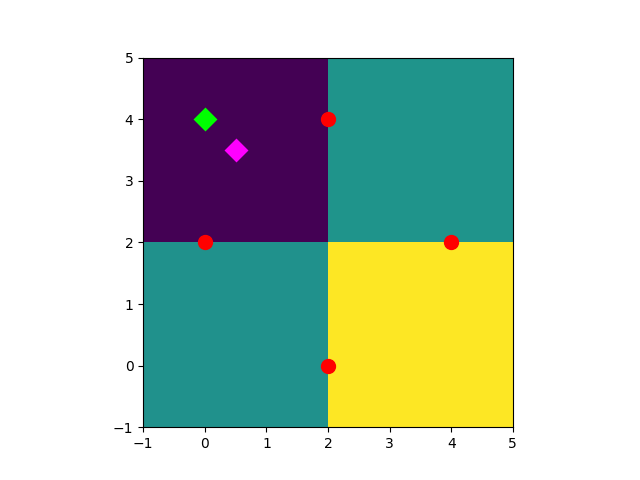
\includegraphics[width=1\linewidth]{images/localizacion7.png}
  \caption{Primera iteración de la localización inicial}
  \label{fig:localizacion_ej1}
\end{figure}
\begin{figure}[htb]
  \centering
  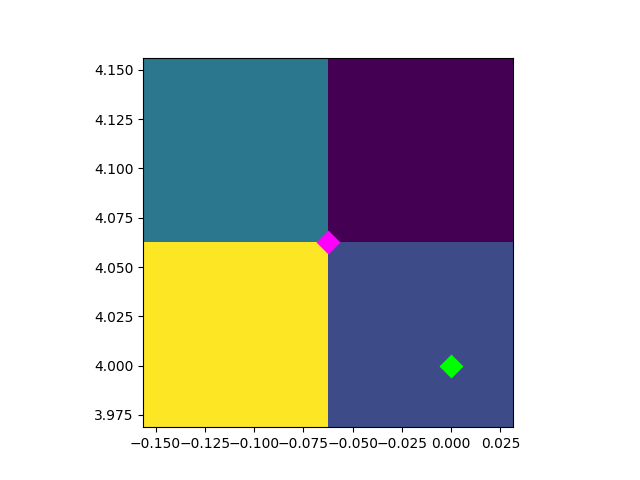
\includegraphics[width=1\linewidth]{images/localizacion8.png}
  \caption{Última iteración de la localización inicial}
  \label{fig:localizacion_ej2}
\end{figure}

\bigskip En la figura \ref{fig:localizacion_ej3} se observa la evolución de la posición real del robot en rojo, así como las correcciones de la posición ideal, en verde. Vemos como cuando la trayectoria predicha se separa lo suficiente de la real, se realiza una corrección.

\begin{figure}[htb]
  \centering
  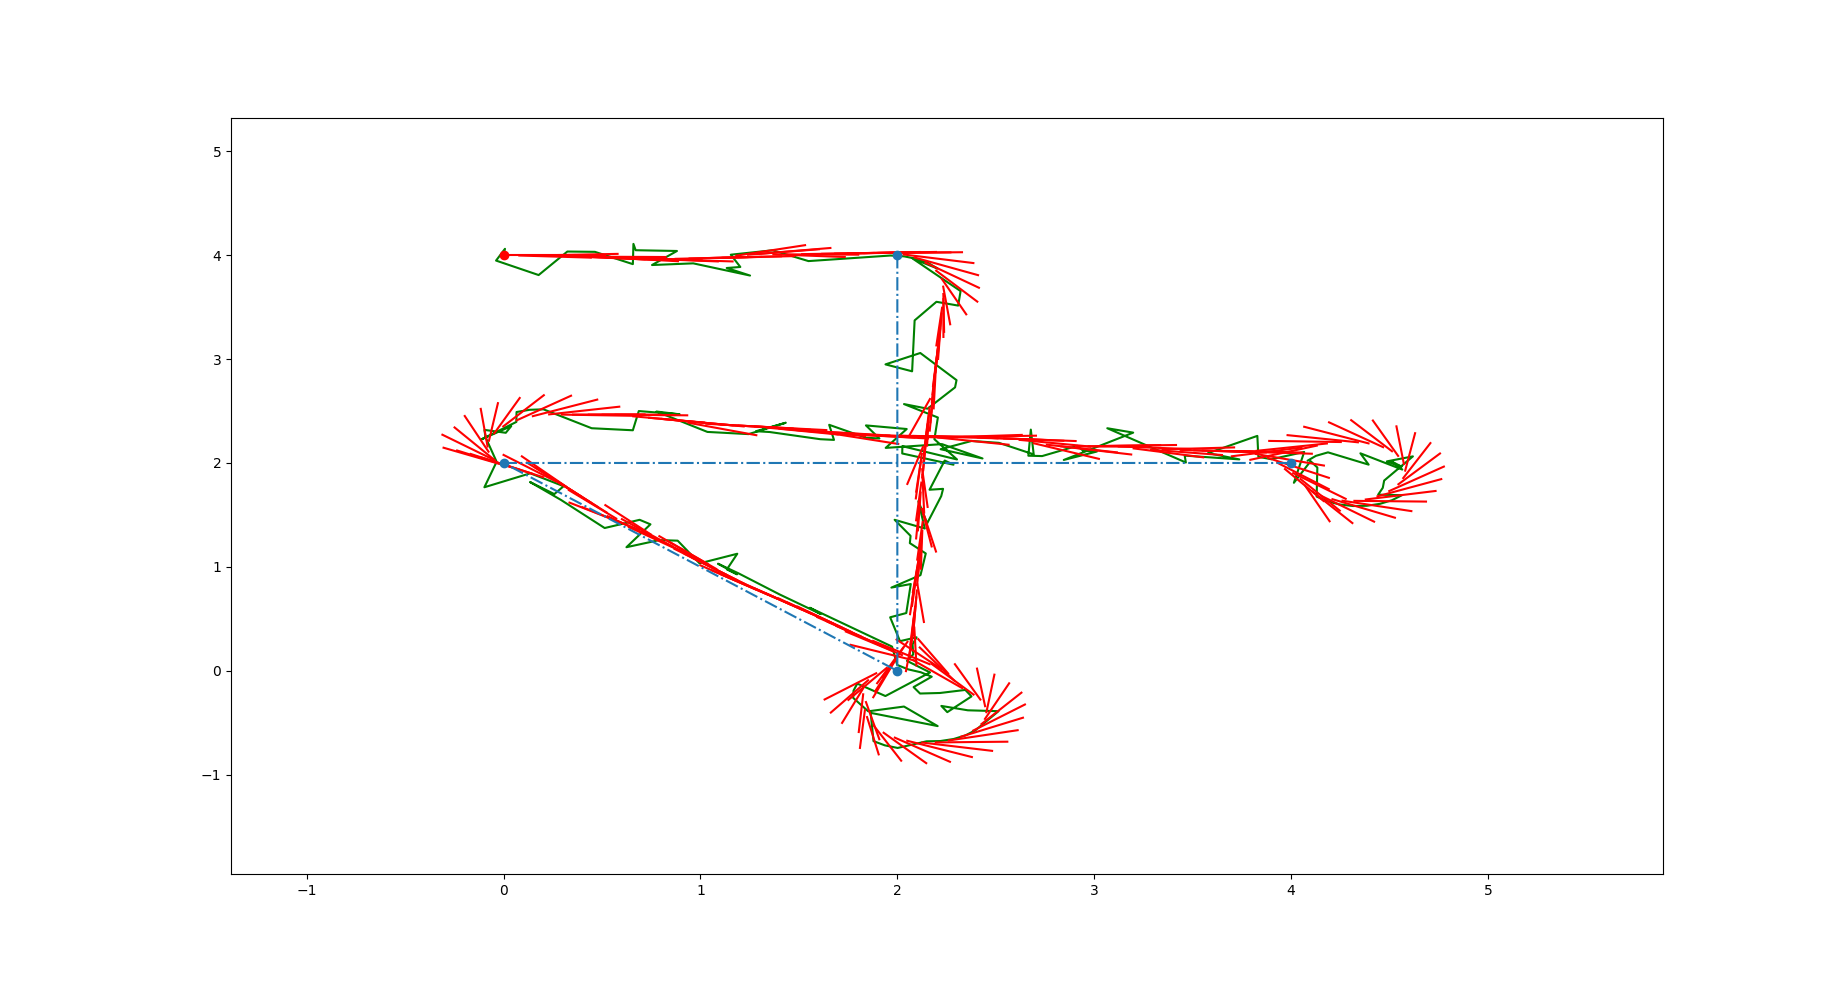
\includegraphics[width=1\linewidth]{images/localizacion9.png}
  \caption{Trayectoria del ejemplo 1}
  \label{fig:localizacion_ej3}
\end{figure}

\subsection{Ejemplo 2}
Mantenemos los valores del experimento anterior, pero disminuimos el umbral a 0.01, lo que debería aumentar la precisión de la trayectoria ideal. En la figura \ref{fig:localizacion_ej4} observamos el resultado de ejecución. Cabe destacar que se han realizado giros alrededor de todas las balizas, incluso varios en el caso de la baliza izquierda. Esto 
es debido a que la trayectoria predicha se ha quedado a una distancia mayor al umbral de las balizas, por lo que se ha tenido que ajustar la trayectoria real para aseguarse de que pasa por las balizas. Además, observamos que la trayectoria ideal, en verde, se reajusta más veces que en el ejemplo 1.
\begin{figure}[htb]
  \centering
  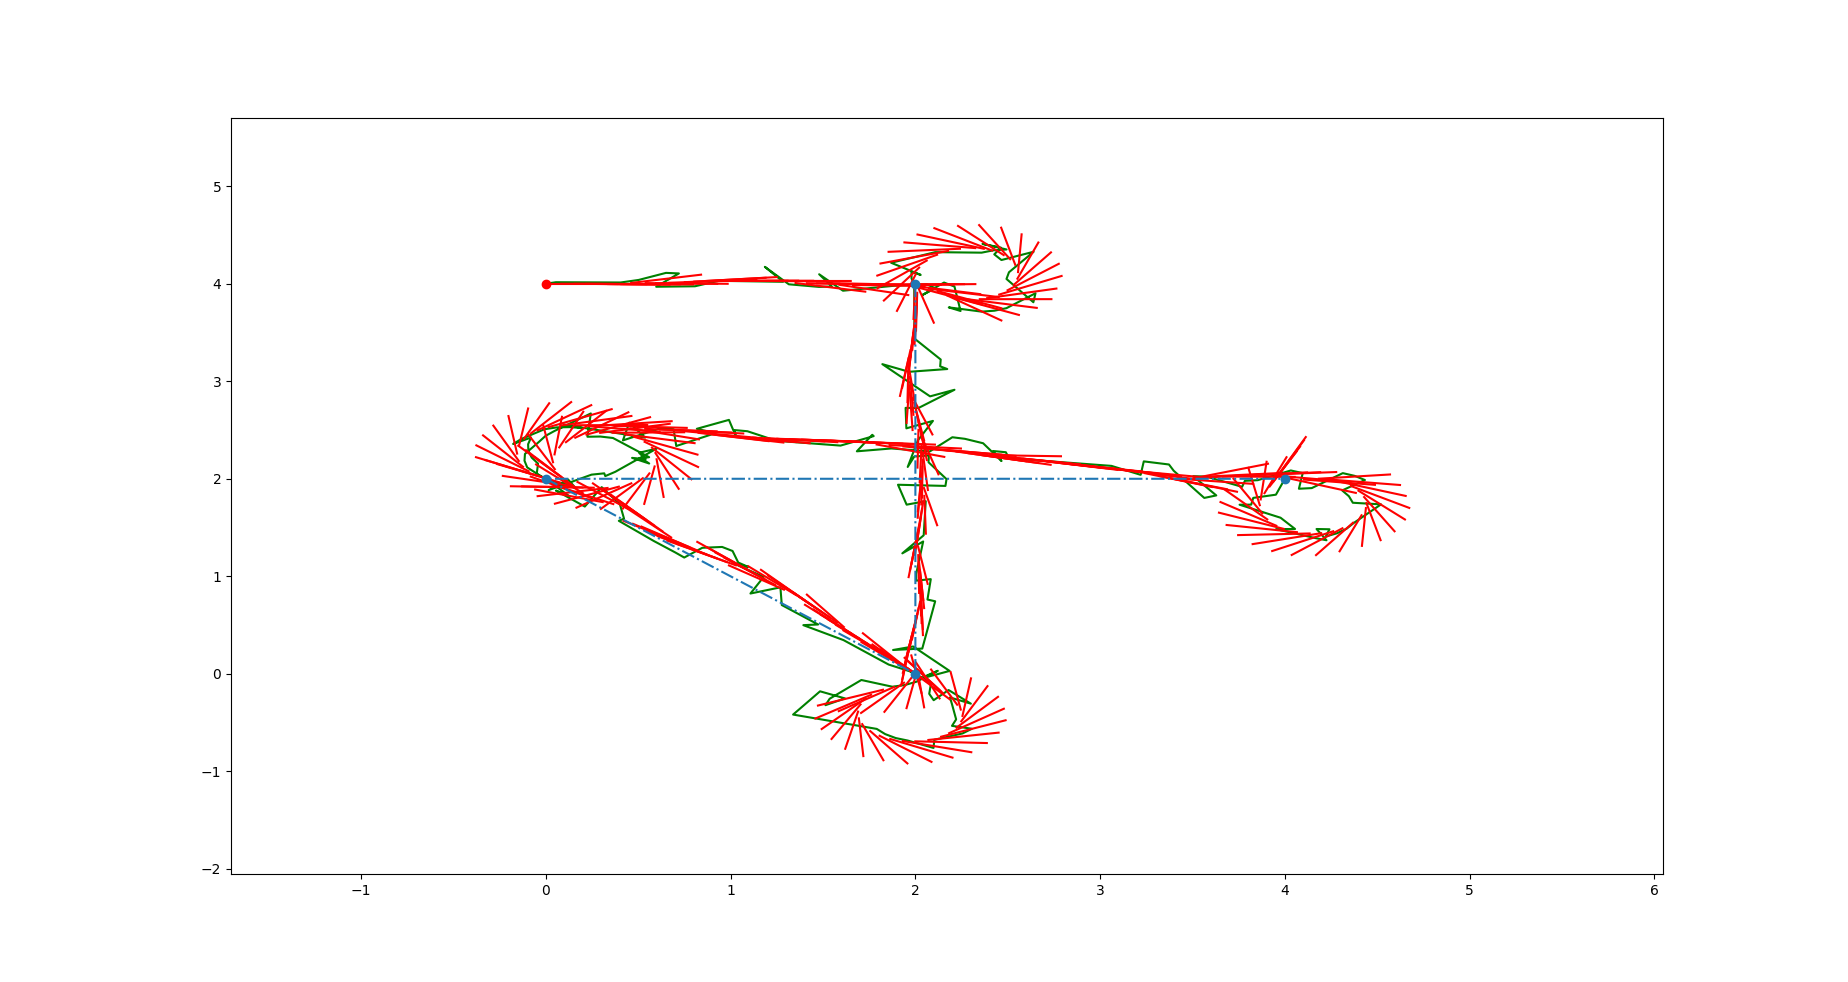
\includegraphics[width=1\linewidth]{images/localizacion10.png}
  \caption{Trayectoria del ejemplo 2}
  \label{fig:localizacion_ej4}
\end{figure}

\subsection{Ejemplo 3}
Ahora consideramos la configuración del ejemplo 2, pero aumentamos la velocidad angular a 240º por segundo (por defecto estaba a 140º/s). 
En la figura \ref{fig:localizacion_ej5} se observa la trayectoria del robot. Constatamos que los giros son más cerrados.

\begin{figure}[htb]
  \centering
  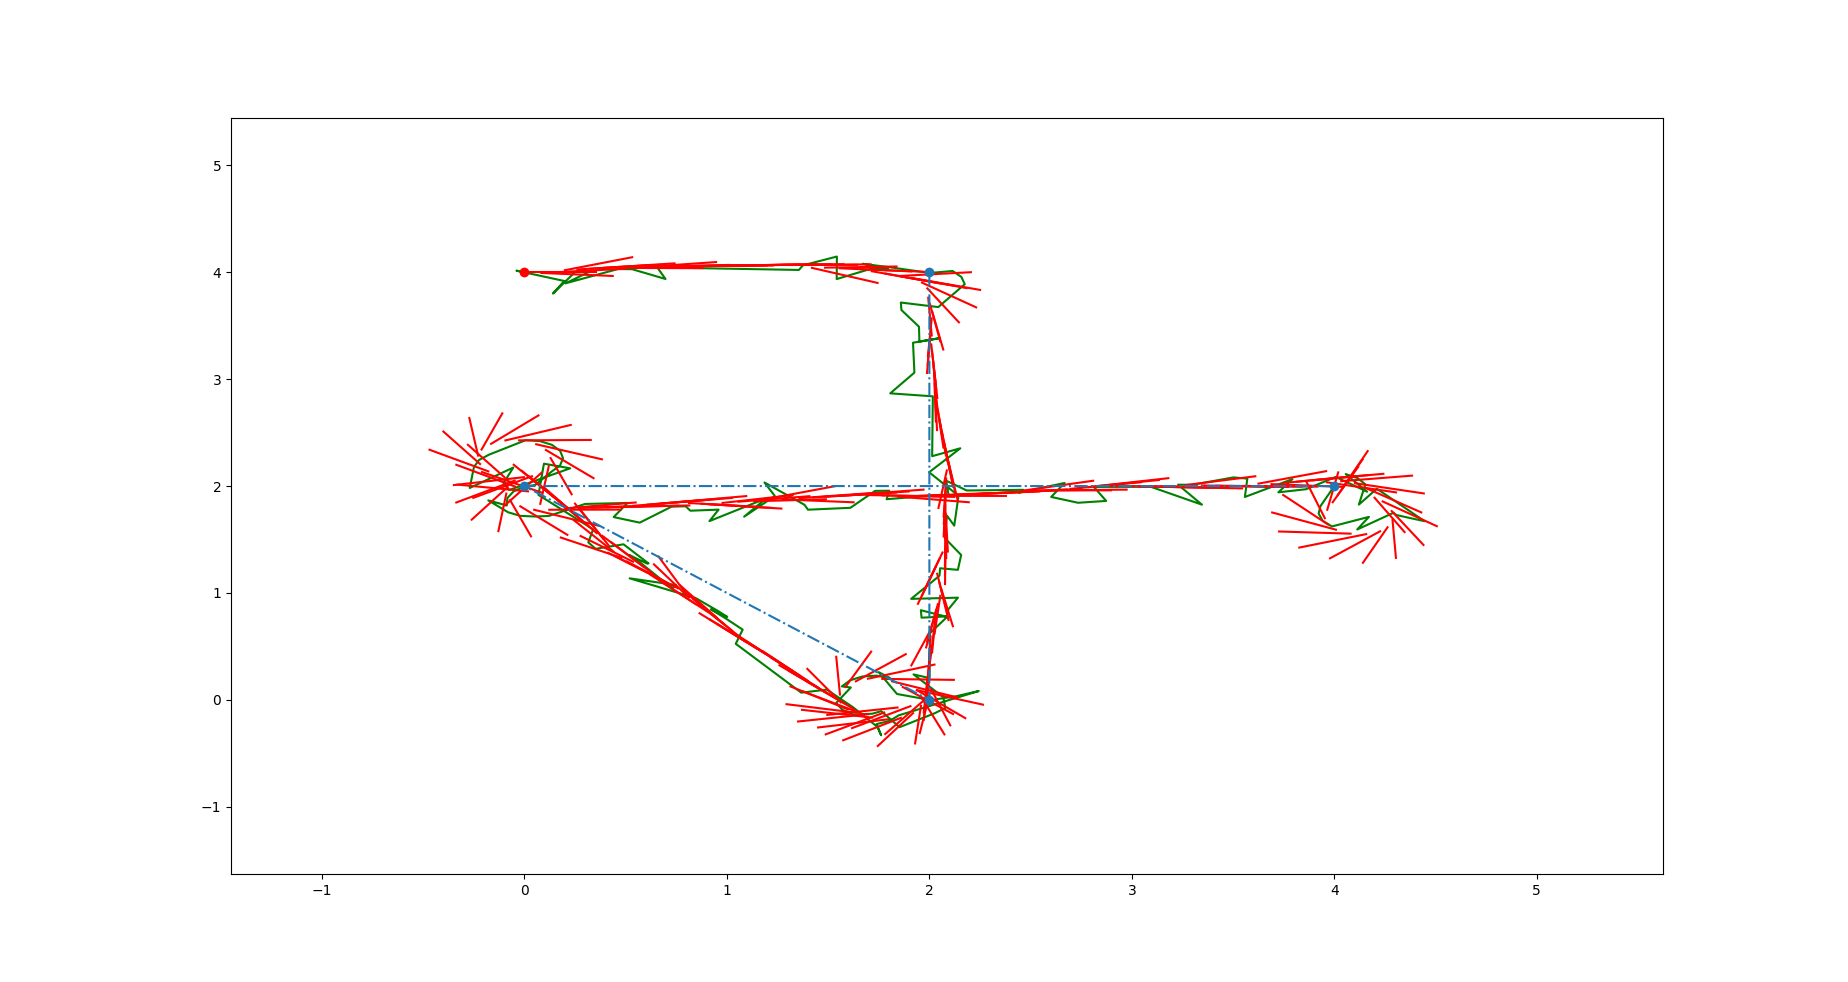
\includegraphics[width=1\linewidth]{images/localizacion11.png}
  \caption{Trayectoria del ejemplo 3}
  \label{fig:localizacion_ej5}
\end{figure}

\subsection{Ejemplo 4}
En este caso mantenemos los valores del ejemplo 2, pero reducimos la velocidad angular a 40º por segundo. 
En la figura \ref{fig:localizacion_ej6} se observa la trayectoria del robot. Vemos que ahora los giros son más abiertos, y en consecuencia, el robot tarda más
en realizar el recorrido y requiere computar más posiciones.

\begin{figure}[htb]
  \centering
  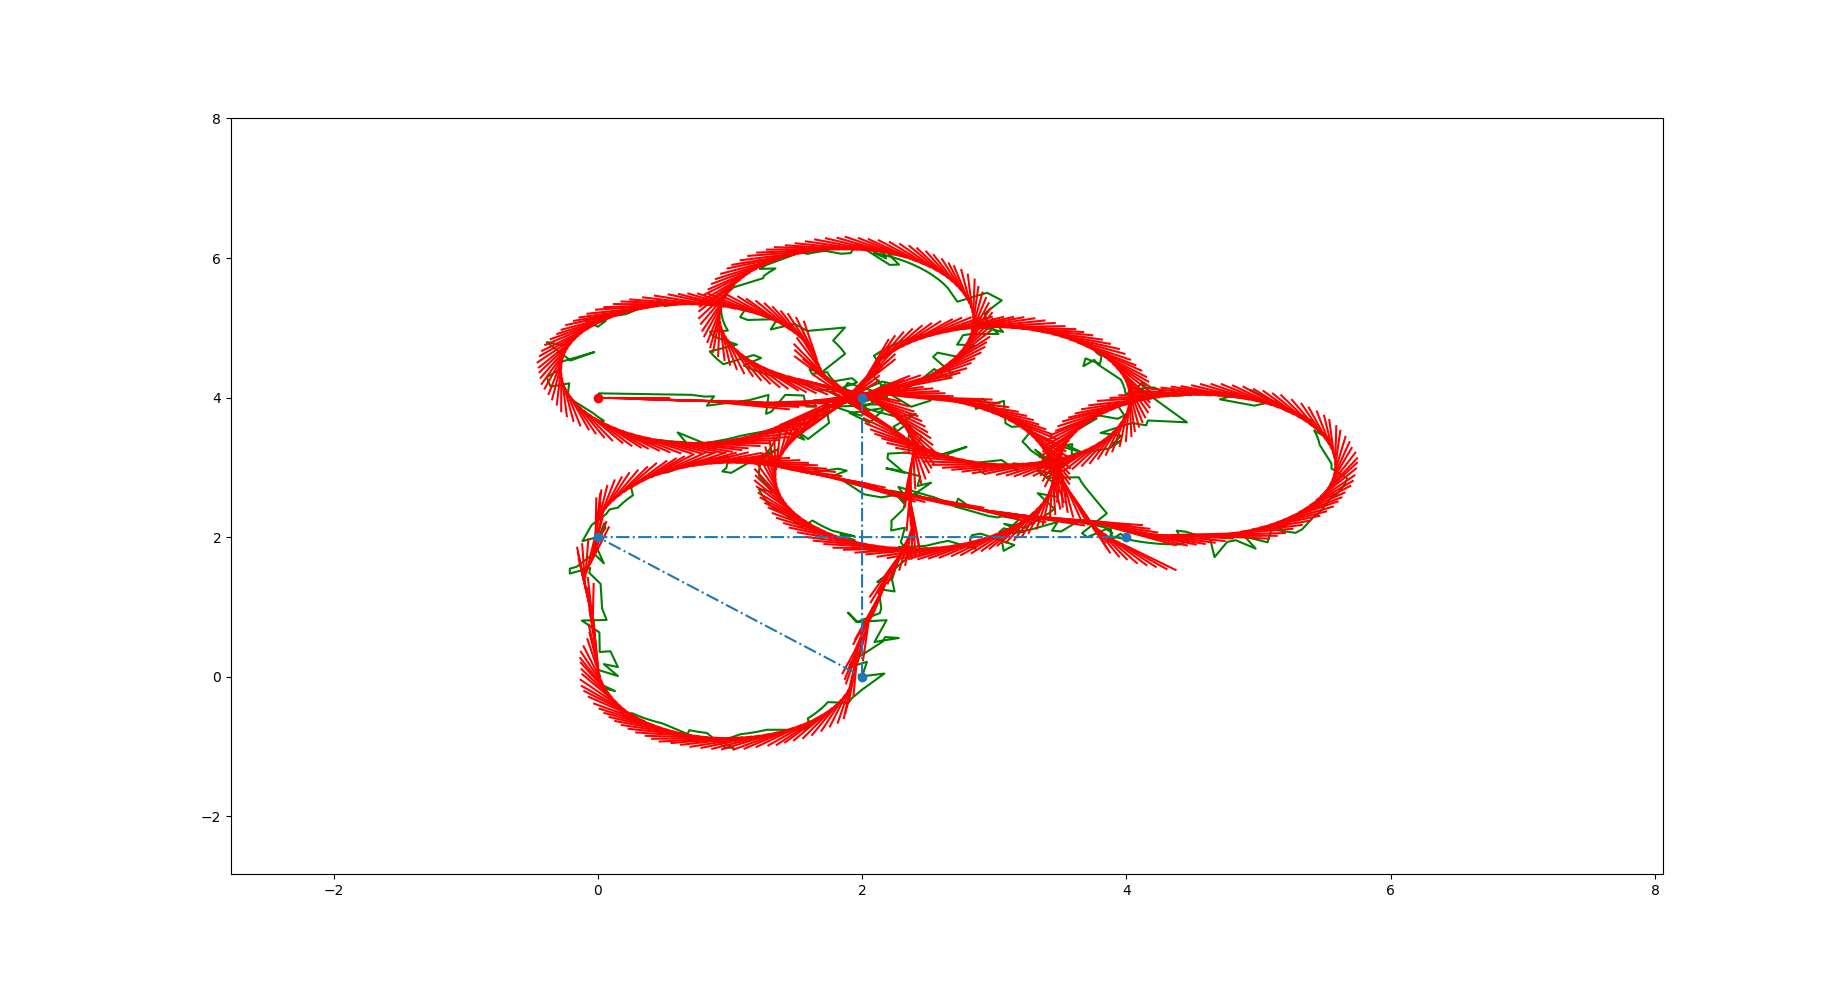
\includegraphics[width=1\linewidth]{images/localizacion12.png}
  \caption{Trayectoria del ejemplo 4}
  \label{fig:localizacion_ej6}
\end{figure}

%%%%%%%%%%%%%%%%%%%%%%%%%%%%%%%%%%%%%%%%%%%%%%%%%%%%%%%%%%%%%
\section{Conclusions}
We have implemented an algorithm for modelling the position and orientation (the pose) of a mobile robot, considering the predicted pose and making adjustments based on sensor measurements regarding the position of beacons.
We have made improvements such as using a variable increment for the search area through a pyramidal approach.

\bigskip Also, we have considered the complexity of the algorithm, which depends on the noise in the movement and sensors, as well as the threshold for the error. A lower threshold requires more calculations, so it is important to find a balance between precision and performance.
This has been proved experimentally. Additionally, we have also tested the impact of the angular velocity on the robot's trajectory, seing that a higher angular velocity results in tighter turns whereas a lower angular velocity results in wider turns and usually a longer trajectory.

\bigskip Although the algorithm has performed well on the experiments, it has a relatively high computational cost, and a more efficient approach will be discussed in the next chapter, the particle filter.
